\documentclass[14pt]{article}
\usepackage[margin=1in]{geometry}
\usepackage{amsmath}
\usepackage{amssymb}
\usepackage{fancyhdr}
\usepackage{graphicx}
\usepackage{xcolor}
\usepackage{tikz}
\usepackage{circuitikz}
\usepackage{hyperref}
\usepackage{subcaption}
\renewcommand{\familydefault}{\sfdefault}
\parindent 0ex
\everymath{\displaystyle{}}
\author{Andy Smit}
\title{ENGG 225\\Fundamentals of Electrical Circuits and Machines}
\date{Winter 2019}


\begin{document}
    \maketitle
    \section{Introduction}
    \subsection{Electric Circuits:}
    The interconnection of circuit elements in a closed path by conductors. 
    The concept of electrical charge is the basics for describing all electrical phenomena. Charge exists in discrete quantities of integer multiples of $1.60\times 10^{-19}C$. In circuit analysis there are two fundamental electrical quantities voltage and current. 
    \subsection{Electical Current:}
    Electrical current is defined as the rate of flow of electrical charges.
    $$i(t)=\frac{d q(t)}{dt}$$
    It is assumed that $i$ is a measure of the equivalent flow of positive charge flow. Given $i(t)$, we can also find $q(t)$
    $$q(t)=\int\limits_{t_0}^t i(t)\, dt+q(t_0)$$
    Normally there is an assigned reference direction for current. Often the direction is unknown and is assumed. The actual direction is determined by the sign of $i$
    \subsubsection{Direct and Alternating Current:}
    \begin{figure}[h]
        \begin{subfigure}[b]{0.5\textwidth}
            
\includegraphics[width=0.95\textwidth]{DirCur.eps}
            \caption{Direct Current}
        \end{subfigure}
        \begin{subfigure}[b]{0.5\textwidth}
            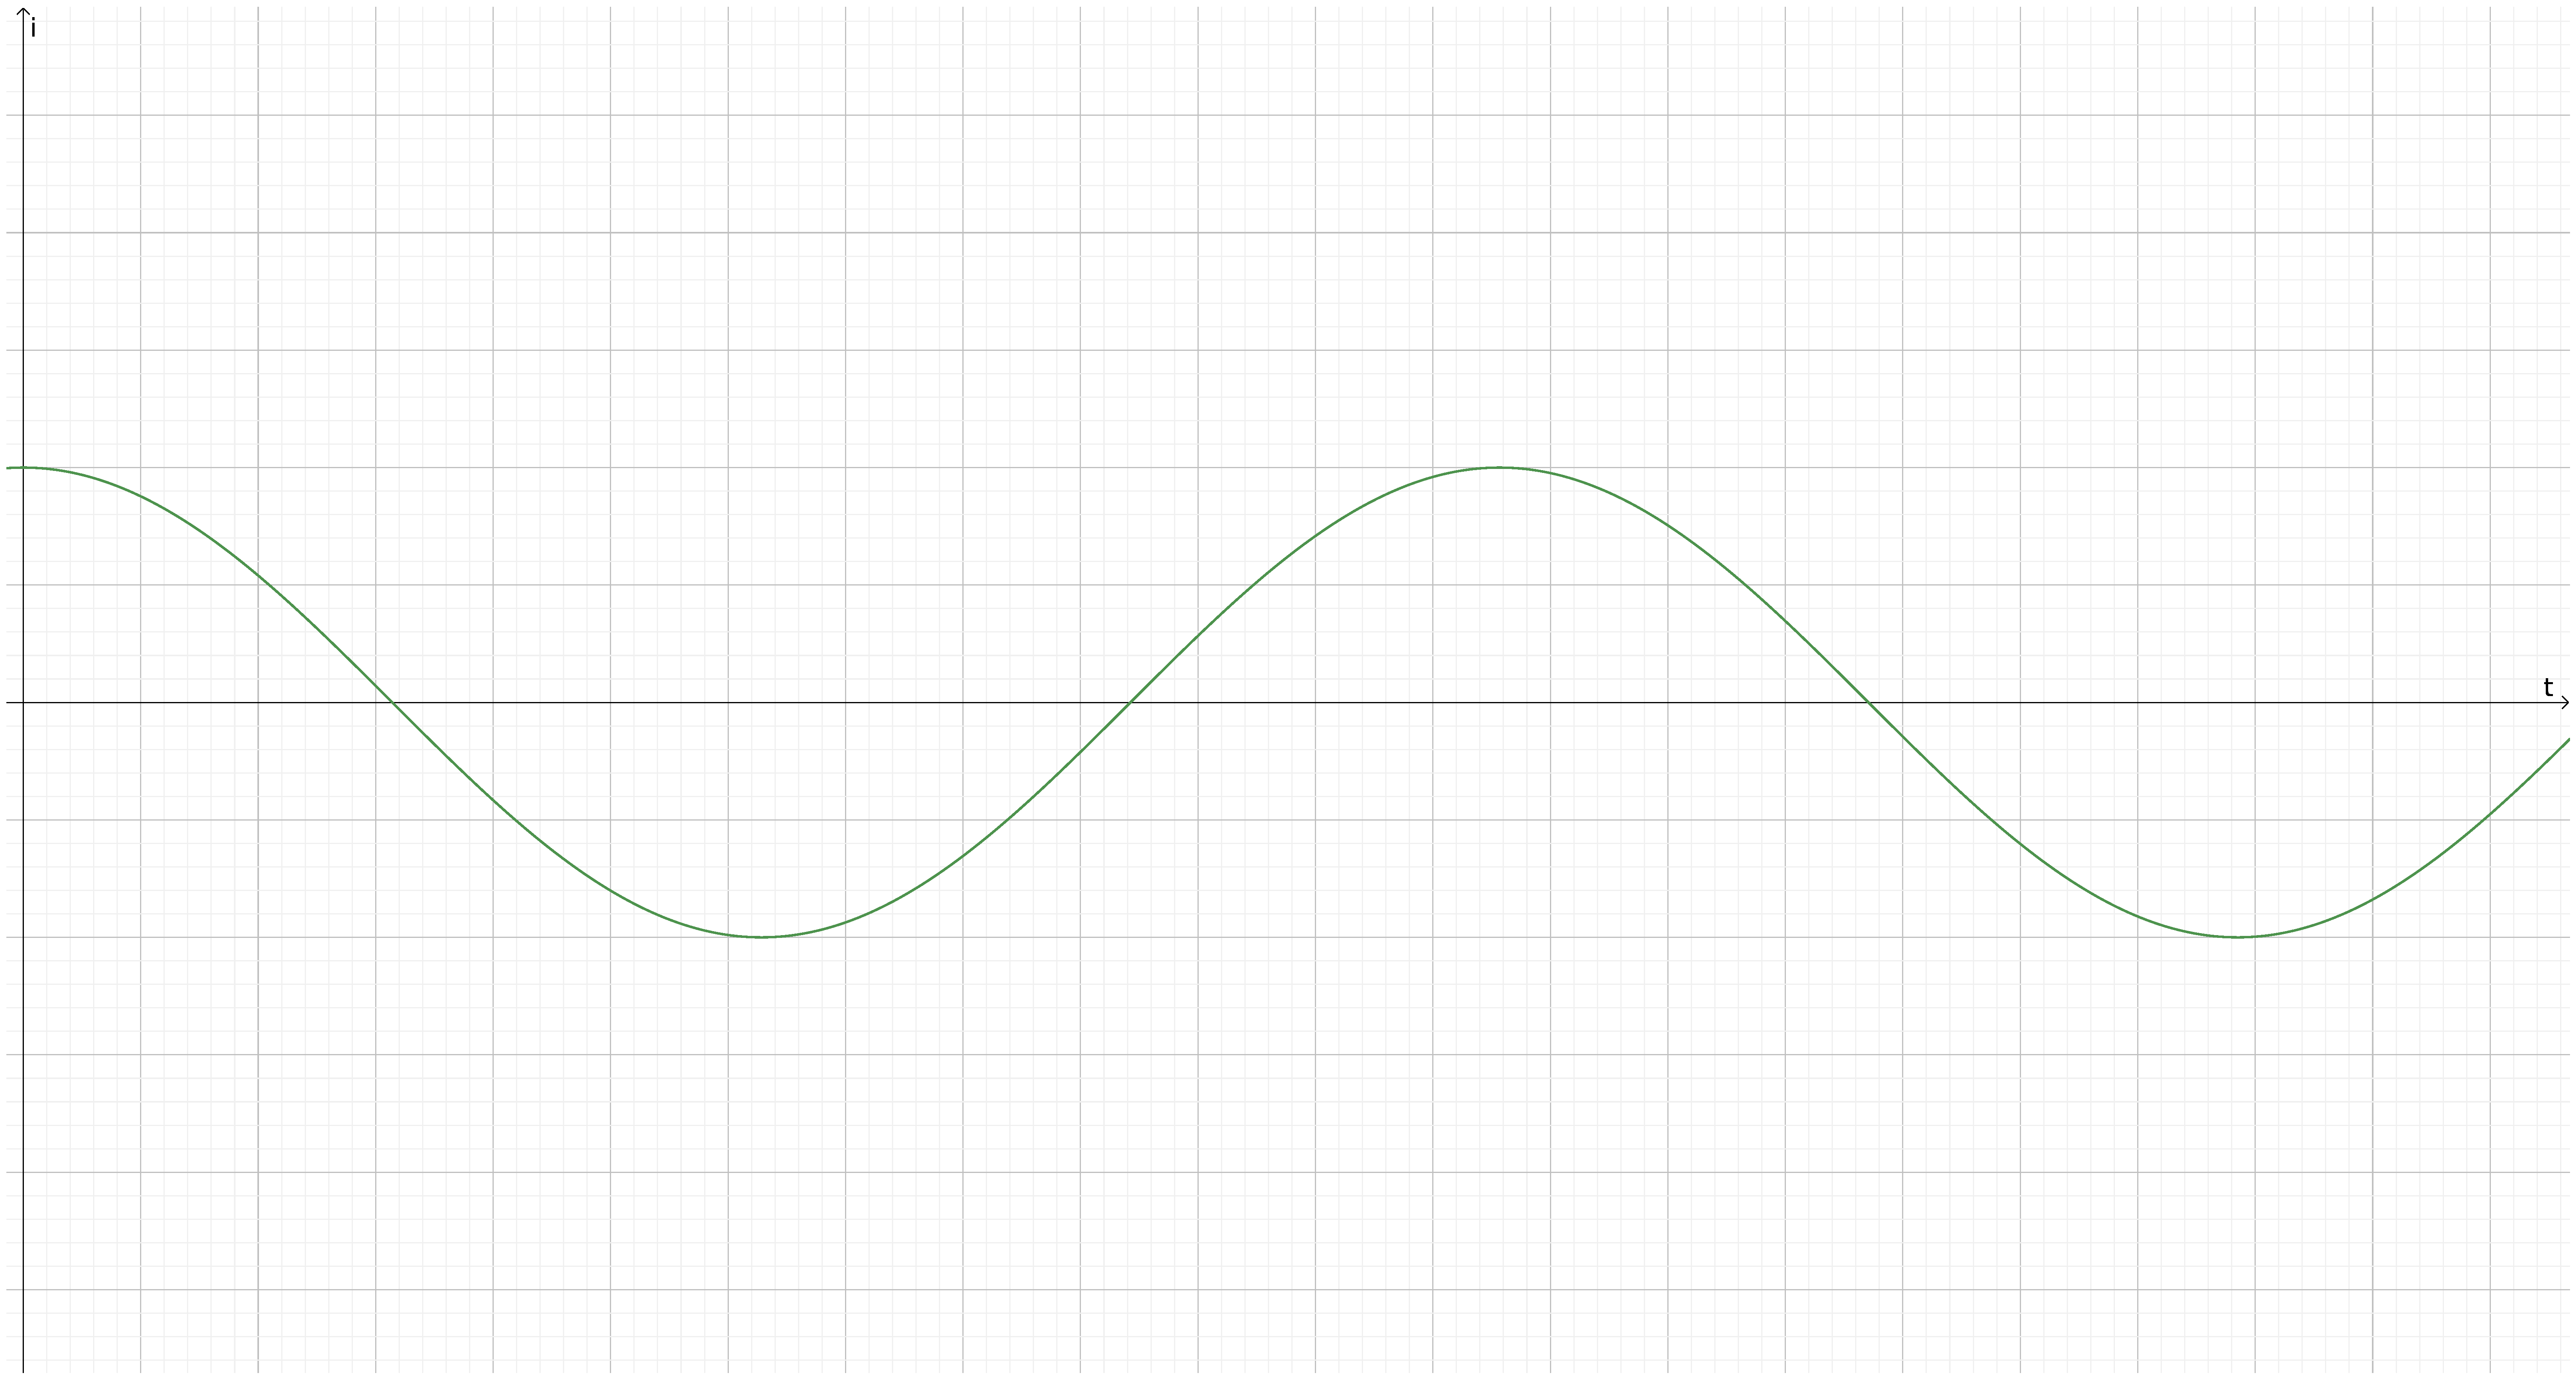
\includegraphics[width=0.95\textwidth]{AltCur.eps}
            \caption{Alternating Current}
        \end{subfigure}
    \end{figure}
    \subsubsection{Notation for Current in Circuit Diagrams}
    \begin{figure}[h]
        \begin{circuitikz}
            \draw (0,0) to[generic, f_>=$i_A$] (2,0);
        \end{circuitikz}
        \caption{Branch Current}
    \end{figure}
    \begin{circuitikz}
        \draw (0,0)node[anchor=east]{$m$} to[generic, f_>=$i_A$] (2,0)node[anchor=west]{$n$};
    \end{circuitikz}
    \section{Resistive Circuits}
    \section{Operational Amplifiers}
    \section{Capacitors and Inductors}
    \section{Sinusoidal Currents and Voltages}  
\end{document}